\section{Results}

\subsection{Skeleton Pruning}

\subsubsection{Kasthuri}

\subsubsection{FlyEM}

\subsection{Classification Performance}

\subsubsection{Kasthuri}

\subsubsection{FlyEM}

\subsection{Graph Based Strategies}

\subsubsection{Kasthuri}

\subsubsection{FlyEM}


%Here we show the results for the three main contributions for this paper: merge consideration using skeleton pruning, merge probabilities output from the trained convolutional neural network, and the final output of the pipeline. 

%\subsection{Skeleton Pruning}

%\subsubsection{Finding Merge Candidates}


%\subsubsection{Finding Split Candidates}

%Effective pruning for merge candidates should have high precision and recall for segments that should be merged.

%\subsection{Neural Network Classification}

%\subsubsection{Merge Network}



%\begin{figure}
%	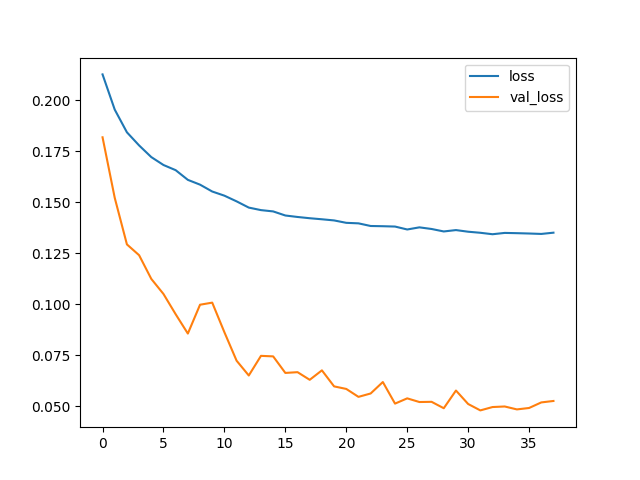
\includegraphics[width=0.85\linewidth]{figures/skeleton-training-curve.png}
%	\caption{The training and validation loss when training the neural network on the L. Cylinder data set.}
%	\label{fig:training-curve}
%\end{figure}

%\begin{figure}
%	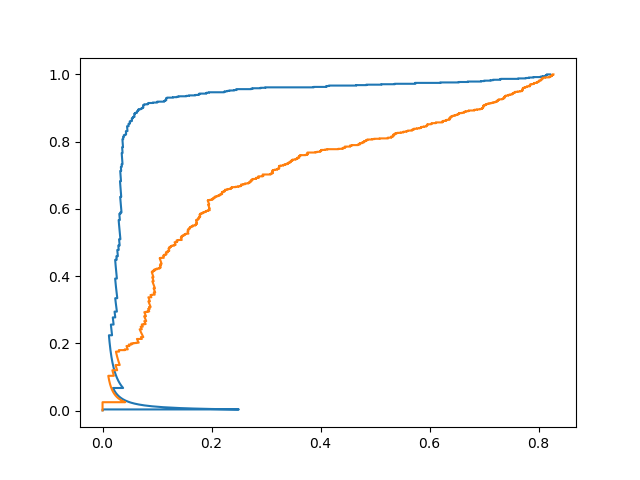
\includegraphics[width=0.85\linewidth]{figures/roc-microns-300-test.png}
%	\caption{The ROC curve for the training and validation datasets.}
%	\label{fig:roc-curve}
%\end{figure}

%Figure \ref{fig:training-curve} shows the training and validation loss during the training of the neural network.

%\begin{figure*}[t]
%	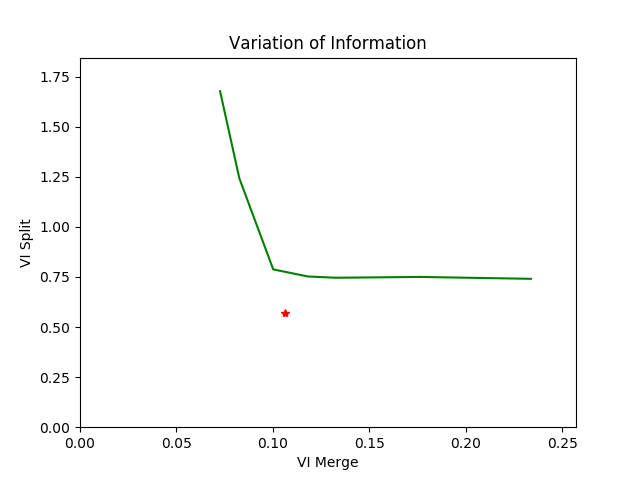
\includegraphics[width=0.45\linewidth]{figures/variation_of_information-train.png}
%	\hspace{0.0825\linewidth}
%	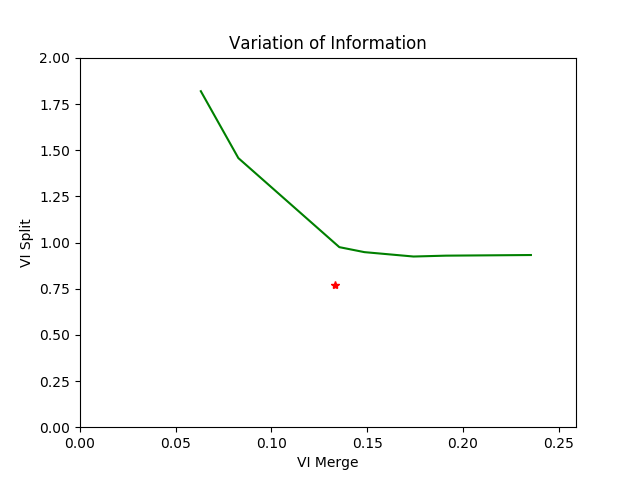
\includegraphics[width=0.45\linewidth]{figures/variation_of_information-test.png}	
%\end{figure*}

%\subsubsection{Split Network}



%\subsection{Graph-based Error Correction}